\documentclass[xcolor={dvipsnames},aspectratio=169,10pt]{beamer}
\usepackage{multimedia}
\input{preamble.tex}

\title{Finding a fETus with UltraSound (FETUS)}
\subtitle{Public Engagement Activities}
\author{
Shu Wang,
Ou Zhanchong, and
{\bf Miguel Xochicale}
}
\date{
Event name {\bf \#2021} \\
6th July 2021
}
\institute{
	\faEnvelope e-mail@server.com \\
	\faGithubAlt @githubhandler \faTwitter @twitterhandler
		}

\titlegraphic{
  \begin{tikzpicture}[overlay, remember picture]
    \node[%
      above right=0.35cm and -0.2cm of current page footer area.south west,
      anchor=south west,
      inner sep=0pt] {%
      \usebeamerfont{footline}
      \begin{tabular}{lm{.8\textwidth}}
        \href{http://creativecommons.org/licenses/by/4.0/}{\ccby} &
        This slices is licensed under a
	\href{http://creativecommons.org/licenses/by/4.0/}
		{Creative Commons ``Attribution 4.0 International''} license. 
	\par Get source of this slides and see further references 
		from \url{https://github.com/ofetus/slides}.
      \end{tabular}
    };
    \node[%
      above left=0.35cm and 0cm of current page footer area.south east,
      anchor=south east,
      inner sep=0pt]{\qrcode[height=1.5cm]{https://github.com/ofetus/repository-name}};
  \end{tikzpicture}
}

\begin{document}

\maketitle

\begin{frame}{Contents}
    \tableofcontents
\end{frame}

%%%%%%%%%%%%%%%%%%%%%%%%%%%%%%%%%%%%%%%%%%%%
\section{Who are we?}

%%%%%%%%%%%%%%%%%%%%%%%%%%%%%%%%%%%%%%%%%%%%%
%\subsection{FETUS}

%%%%%%%%%%%%%%%%%%%%%%%%%%%%%%%%%%%%%%%%%%%%%%%%%%%%%%%%
{
%\paper{Lastname N. YEAR in journal of...}
\begin{frame}{Who are we? / Where we come from? / Do we have hobbies?}

  \begin{figure}
  \centering
  \includegraphics[width=1.0\textwidth]{./figures/who-we-are/versions/drawing-v01.png}
  \end{figure}

\end{frame}
}


%%%%%%%%%%%%%%%%%%%%%%%%%%%%%%%%%%%%%%%%%%%%
\section{Guessing Fetal Growth}

%%%%%%%%%%%%%%%%%%%%%%%%%%%%%%%%%%%%%%%%%%%%%
%\subsection{FETUS}

%%%%%%%%%%%%%%%%%%%%%%%%%%%%%%%%%%%%%%%%%%%%%%%%%%%%%%%%
{
\paper{Growing Baby: 3D Print-ready Models}
\begin{frame}{Can you guess the *AGE* of these fetus?}
      \begin{figure}
        \centering
        \includegraphics[width=1.0\textwidth]{./figures/fetal-ages/versions/drawing-v00.png}
        %\caption{}
      \end{figure}
\end{frame}
}

%%%%%%%%%%%%%%%%%%%%%%%%%%%%%%%%%%%%%%%%%%%%%%%%%%%%%%%%
{
\paper{Growing Baby: 3D Print-ready Models}
\begin{frame}{Can you guess the *AGE* of these fetus?}
      \begin{figure}
        \centering
        \includegraphics[width=1.0\textwidth]{./figures/fetal-ages/versions/drawing-v01.png}
        %\caption{}
      \end{figure}
\end{frame}
}

%%%%%%%%%%%%%%%%%%%%%%%%%%%%%%%%%%%%%%%%%%%%%%%%%%%%%%%%
{
\paper{ de Bakker et al. 2016 in Science \url{http://3datlas.3dembryo.nl/}; \url{https://www.whattoexpect.com/pregnancy/}}
\begin{frame}{Can you guess the *SIZE* of these fetus?}
      \begin{figure}
        \centering
        \includegraphics[width=1.0\textwidth]{./figures/fetal-size/versions/drawing-v00.png}
        %\caption{}
      \end{figure}
\end{frame}
}



%%%%%%%%%%%%%%%%%%%%%%%%%%%%%%%%%%%%%%%%%%%%
\section{Looking inside the human body}

%%%%%%%%%%%%%%%%%%%%%%%%%%%%%%%%%%%%%%%%%%%%%
%\subsection{FETUS}
%Medical imaging in pregnancy

%%%%%%%%%%%%%%%%%%%%%%%%%%%%%%%%%%%%%%%%%%%%%%%%%%%%%%%%
{
\paper{\url{https://en.wikipedia.org/wiki/Medical_imaging_in_pregnancy}}
\begin{frame}{Medical Imaging in Pregnancy}
      \begin{figure}
        \centering
        \includegraphics[width=1.0\textwidth]{./figures/medical-imaging/versions/drawing-v01.png}
        %\caption{}
      \end{figure}
\end{frame}
}


%%%%%%%%%%%%%%%%%%%%%%%%%%%%%%%%%%%%%%%%%%%%%%%%%%%%%%%%
{

\paper{Fetal and Mother Numerical Models (FEMONUM) in \url{http://femonum.telecom-paristech.fr}}
%https://perso.telecom-paristech.fr/angelini/projects_research/FEMONUM/femonum_en.html
%https://perso.telecom-paristech.fr/angelini/projects_research/FEMONUM/femonum_en.html

\begin{frame}{Modelling US imaging}
      \begin{figure}
        \centering
        \includegraphics[width=1.0\textwidth]{./figures/modelling-us-imaging/versions/drawing-v01.png}
        %\caption{}
      \end{figure}
\end{frame}
}



%%%%%%%%%%%%%%%%%%%%%%%%%%%%%%%%%%%%%%%%%%%%%%%%%%%%%%%%
{
%\paper{3D printing FETUS}
\begin{frame}{3D printing FETUS}
      \begin{figure}
        \centering
        \includegraphics[width=1.0\textwidth]{./figures/3d-printing/versions/drawing-v00.png}
        %\caption{}
      \end{figure}
\end{frame}
}

%%%%%%%%%%%%%%%%%%%%%%%%%%%%%%%%%%%%%%%%%%%%%%%%%%%%%%%%
{
\begin{frame}
  \frametitle{Example 1}
  \vspace{10pt}
  \begin{center}
    \movie{\includegraphics[width=0.5\textwidth]{./figures/apollo/apollo17.jpg}}{./figures/apollo/apollo17.avi}
  \end{center}

  \begin{itemize}
    \item Click on the image to play/pause the video.
    \item Move pointer to the bottom of the video frame for a draggable position
      control.
  \end{itemize}
\end{frame}
}

%%%%%%%%%%%%%%%%%%%%%%%%%%%%%%%%%%%%%%%%%%%%
\section{Simulator for Ultrasound-Guidance Interventions}

%%%%%%%%%%%%%%%%%%%%%%%%%%%%%%%%%%%%%%%%%%%%%%%%%%%%%%%%
{
\paper{(a) Coordinate systems overview sketch in 3D Slicer,  (b) Asselin et al. 2018 in conf-BIVPCS, (c) US-simulator, and (d) 3D-printed fetus}
\begin{frame}{Simulator for Ultrasound-Guidance Interventions}

  \begin{columns}
    \begin{column}{.3\linewidth}
      Towards a more realistic
  \begin{itemize}
    \item \textbf{UGI}
    \item \textbf{US images}
    \item \textbf{Phantoms with 3D-printed US compatible material}
    \item \textbf{Training for in-plane, out-of-plane needle tracking}
  \end{itemize}

    \end{column}


  \begin{column}{.6\linewidth}

      \begin{figure}
        \centering
        \includegraphics[width=0.9\textwidth]{./figures/simulator-for-ugi/versions/drawing-v01.png}
      \end{figure}

    \end{column}
  \end{columns}


\end{frame}
}

%%%%%%%%%%%%%%%%%%%%%%%%%%%%%%%%%%%%%%%%%%%%
\section{Takeaway messages / Pop Quiz / Surprises }

%\subsection{Takeaway messages}
%\subsection{Surprises}
%\subsection{5 minutes Evaluation}


%%%%%%%%%%%%%%%%%%%%%%%%%%%%%%%%%%%%%%%%%%%%%%%%%%%%%%%%
{
%\paper{Lastname N. YEAR in journal of...}
\begin{frame}{Takeaway messages}
  \begin{figure}
  \centering
  \includegraphics[width=1.0\textwidth]{./../figures/takeaways/versions/drawing-v04}
  \end{figure}

\end{frame}
}

%%%%%%%%%%%%%%%%%%%%%%%%%%%%%%%%%%%%%%%%%%%%%%%%%%%%%%%%
{
%\paper{Lastname N. YEAR in journal of...}
\begin{frame}{Pop Quiz and Souvenirs}
  \begin{figure}
  \centering
  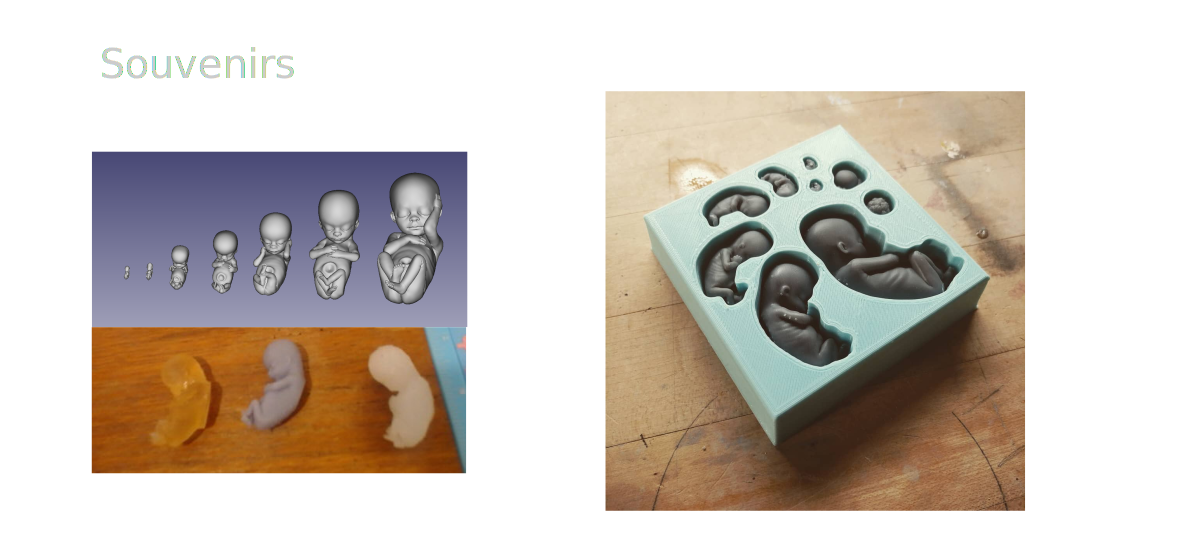
\includegraphics[width=1.0\textwidth]{./../figures/popquiz-souvenirs/versions/drawing-Ss-v02}
  \end{figure}

\end{frame}
}


%%%%%%%%%%%%%%%%%%%%%%%%%%%%%%%%%%%%%%%%%%%%%%%%%%%%%%%%
{
%\paper{Lastname N. YEAR in journal of...}
\begin{frame}{Pop Quiz and Souvenirs}
  \begin{figure}
  \centering
  \includegraphics[width=1.0\textwidth]{./../figures/popquiz-souvenirs/versions/drawing-Qs-v01}
  \end{figure}

\end{frame}
}


%%%%%%%%%%%%%%%%%%%%%%%%%%%%%%%%%%%%%%%%%%%%%%%%%%%%%%%%
{
%\paper{Lastname N. YEAR in journal of...}
\begin{frame}{Extra Questions (EQ)}
  \begin{figure}
  \centering
  \includegraphics[width=1.0\textwidth]{./../figures/popquiz-souvenirs/versions/drawing-Qs2-v00}
  \end{figure}

\end{frame}
}



%%%%%%%%%%%%%%%%%%%%%%%%%%%%%%%%%%%%%%%%%%%%%%%%%%%%%%%%
{
%\paper{Lastname N. YEAR in journal of...}
\begin{frame}{Acknowledgements}

  \begin{figure}
  \centering
  \includegraphics[width=1.0\textwidth]{./../figures/team/versions/drawing-v05.png}
  \end{figure}

\end{frame}
}


%\begin{frame}[standout]
%  Thanks \\
%  Questions?
%\end{frame}

\maketitle

\end{document}
